\documentclass{article}
\usepackage{tikz}

\begin{document}
\begin{center}
\textbf{\large Hierarchy of Linux Distribution}\\
\end{center}

\begin{figure}[h]
\centering
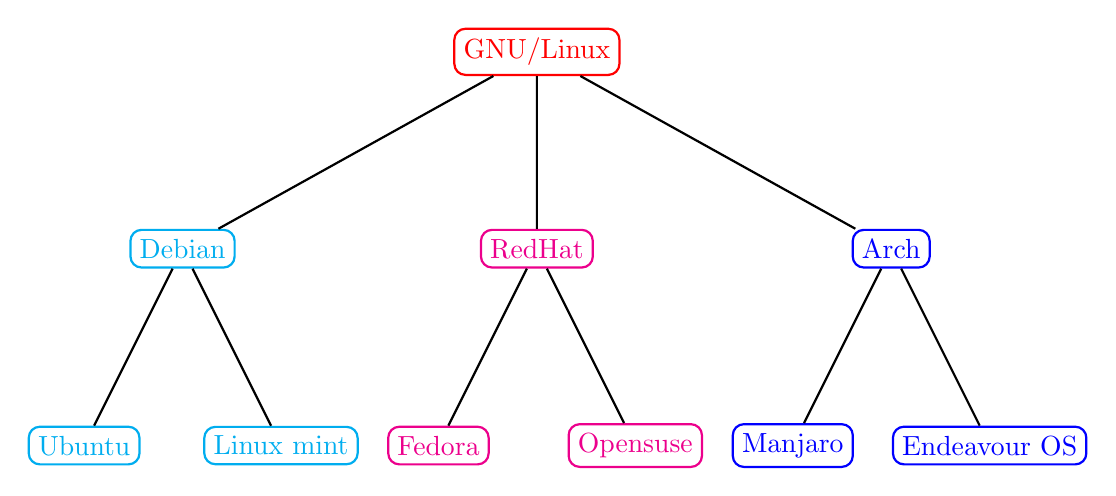
\begin{tikzpicture}[every node/.style={shape=rectangle, rounded corners, draw, align=center}]
\path [draw,thick,-]
node (root)[red] {GNU/Linux}
[sibling distance = 45mm, level distance =25mm]
child{ node [cyan] {Debian}
[sibling distance = 25mm, level distance =25mm]
child{ node [cyan] {Ubuntu} }
child{ node [cyan] {Linux mint} }
} 
child{ node [magenta] {RedHat}
[sibling distance = 25mm, level distance =25mm]
child{ node [magenta] {Fedora} }
child{ node [magenta] {Opensuse} }
} 
child{ node [blue] {Arch}
[sibling distance = 25mm, level distance =25mm]
child{ node [blue] {Manjaro} }
child{ node [blue] {Endeavour OS} }
};
\end{tikzpicture}
\caption{GNU/Linux Operating System Family}
\end{figure}

\pagebreak

\begin{center}
\textbf{\large SUV Cars}
\end{center}

\begin{figure}[h]
\centering
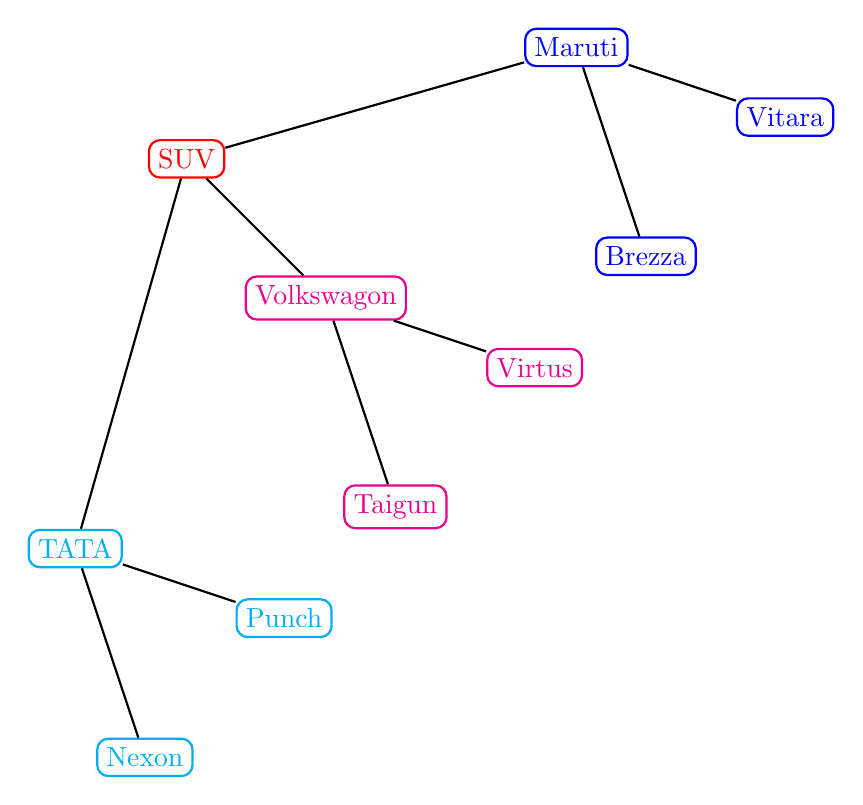
\begin{tikzpicture}[every node/.style={shape=rectangle, rounded corners, draw, align=center}]
\path [draw, thick, -] 
[grow=-45]
node(root)[red]{SUV}
[sibling distance=45mm, level distance=25mm]
child{node[cyan]{TATA}[sibling distance=25mm, level distance=25mm]
child{node[cyan]{Nexon}} 
child{node[cyan]{Punch}}
}
child{node[magenta]{Volkswagon}
[sibling distance=25mm, level distance=25mm]
child{node[magenta]{Taigun}} 
child{node[magenta]{Virtus}}
}
child{node[blue]{Maruti} [sibling distance=25mm, level distance=25mm]
child{node[blue]{Brezza}} 
child{node[blue]{Vitara}}
};
\end{tikzpicture}
\caption{Car Brands Hierarchy}
\end{figure}
\end{document}
